%!TEX root = ../document.tex
\chapter{Vorbereitung}
\subsubsection*{Von: Marco Egner}
In diesem Kapitel soll erläutert werden, wie das Web-Projekt bereitgestellt und benutzt wird. Hierzu folgt eine kurze Anleitung um einen Host zu installieren, der die Web-Applikation bereitstellt sowie eine Beschreibung mit dem Umgang der bereits installierten virtuellen Maschine. Die empfohlene Installationsweise ist die Installation mit Docker, beschrieben in Kapitel \ref{sec:InstallWithDocker}. 

\section{Installationsanleitung ohne Docker}
\label{sec:Install}

Für die Installation der Web-Applikation ohne den Docker-Container zu nutzen, muss zuerst ein Webserver auf dem Linux Host-Gerät installiert werden, wie z. B. der Apache Server (\url{https://httpd.apache.org}). Eine einfach Installation ist mit dem Befehl \colorbox{altgray}{\lstinline|apt-get install apache2|} möglich. Da sich das Installations-Vorgehen mit den Versionen der Drittanbieter-Software ändert, verzichte ich hier auf eine detaillierte Schritt-für-Schritt-Anleitung. Damit das Webprojekt richtig ausgeführt wird, muss in der apache2.conf folgende zwei Zeilen eingefügt werden:\medskip

\begin{itemize}
	\item \bashCommand{RemoveHandler .html .htm}
	\item \bashCommand{AddType application/x-httpd-php .php .htm .html}\medskip
\end{itemize}
	
Diese Konfiguration sorgt dafür, dass HTML-Seiten mit dem PHP-Interpreter ausgeführt werden. Nach der Konfiguration des Apache-Webservers, muss der PHP-Interpreter installiert werden, dies kann ebenfalls mit dem Package-Manager durchgeführt werden. Dazu wird das Kommando \colorbox{altgray}{\lstinline|apt-get install php|} verwendet. Zum Zeitpunkt der Entwicklung des Projekts, wurde die PHP-Version 7.0.19 verwendet. Um die Installation auf Korrektheit zu prüfen, kann der Befehl \colorbox{altgray}{\lstinline|php --version|} benutzt werden. Dieser zeigt die Versionsnummer der PHP-Umgebung, falls die Installation korrekt durchgeführt wurde.\medskip

Um alle Tutorials durchführen zu können muss der Host einen GNU-Debugger (GDB) bereitstellen. Dieser kann leicht mit  \colorbox{altgray}{\lstinline|apt-get install gdb|} bezogen werden. Um den GDB zu testen, kann der Befehl \colorbox{altgray}{\lstinline|gdb --version|} ausgeführt und die Version angezeigt werden.\medskip

Zuletzt muss noch eine MySQL-Datenbank auf dem Host-System installiert werden. Hierfür stehen mehrere Alternative Vorgehensweisen zur Verfügung, siehe dazu \url{https://dev.mysql.com/doc/refman/5.7/en/linux-installation.html}. Anschließend muss man das MySQL-Skript zur Initialisierung ausführen, dies ist mit dem folgenden Kommando möglich:\\ \colorbox{altgray}{\lstinline|mysql < PROJEKTROOT/Projekte/Docker/server/initalizeDB.sql|} \medskip

Um nun die Applikation verwenden zu können, müssen zunächst alle Web-Ressourcen aus dem GitHub-Repository in den von Apache erwarteten Pfad kopieren. Dazu muss das Repository auf den Server kopiert werden, dies kann mit dem Befehl:\\ \colorbox{altgray}{\lstinline|git clone https://github.com/th-ingolstadt/INF-M-Projekt-Security-Workbench.git|} erreicht werden. Danach muss der Inhalt des Pfads PROJEKTROOT/Projekte/SecWorkbench/html in das Root-Verzeichnis des Apache-Servers kopiert werden. Dieser ist standardmäßig /var/www/html. Zusätzlich muss man die Buffer overflow Programme FirstExample.c und SecondExample.c kompilieren. Hierfür werden die folgenden Befehle genutzt:

\begin{itemize}
	\item \bashCommand{gcc -ggdb /var/www/html/SecWorkbench/App\_Data/FirstExample.c -o}\\ \bashCommand{/var/www/html/SecWorkbench/App\_Data/FirstExample}
	\item \bashCommand{gcc -ggdb /var/www/html/SecWorkbench/App\_Data/SecondExample.c -o}\\ \bashCommand{/var/www/html/SecWorkbench/App\_Data/SecondExample}
\end{itemize}

Des Weiteren müssen die Rechte des Apache-Users auf das Verzeichnis angepasst werden, dies ist mit dem folgenden Befehl möglich \colorbox{altgray}{\lstinline|sudo chown -R www-data:www-data /var/www/html/|}.\medskip

Nun kann die Website testweise ausgeführt werden. Dazu gibt man im Browser in der VM folgende Adresse an:  \colorbox{altgray}{\lstinline|http://localhost/SecWorkbench|}. Es sollte nun die Startseite des Projekts angezeigt werden, siehe dazu Abbildung \ref{fig:startseite}.

\begin{figure}[H]
	\centering
	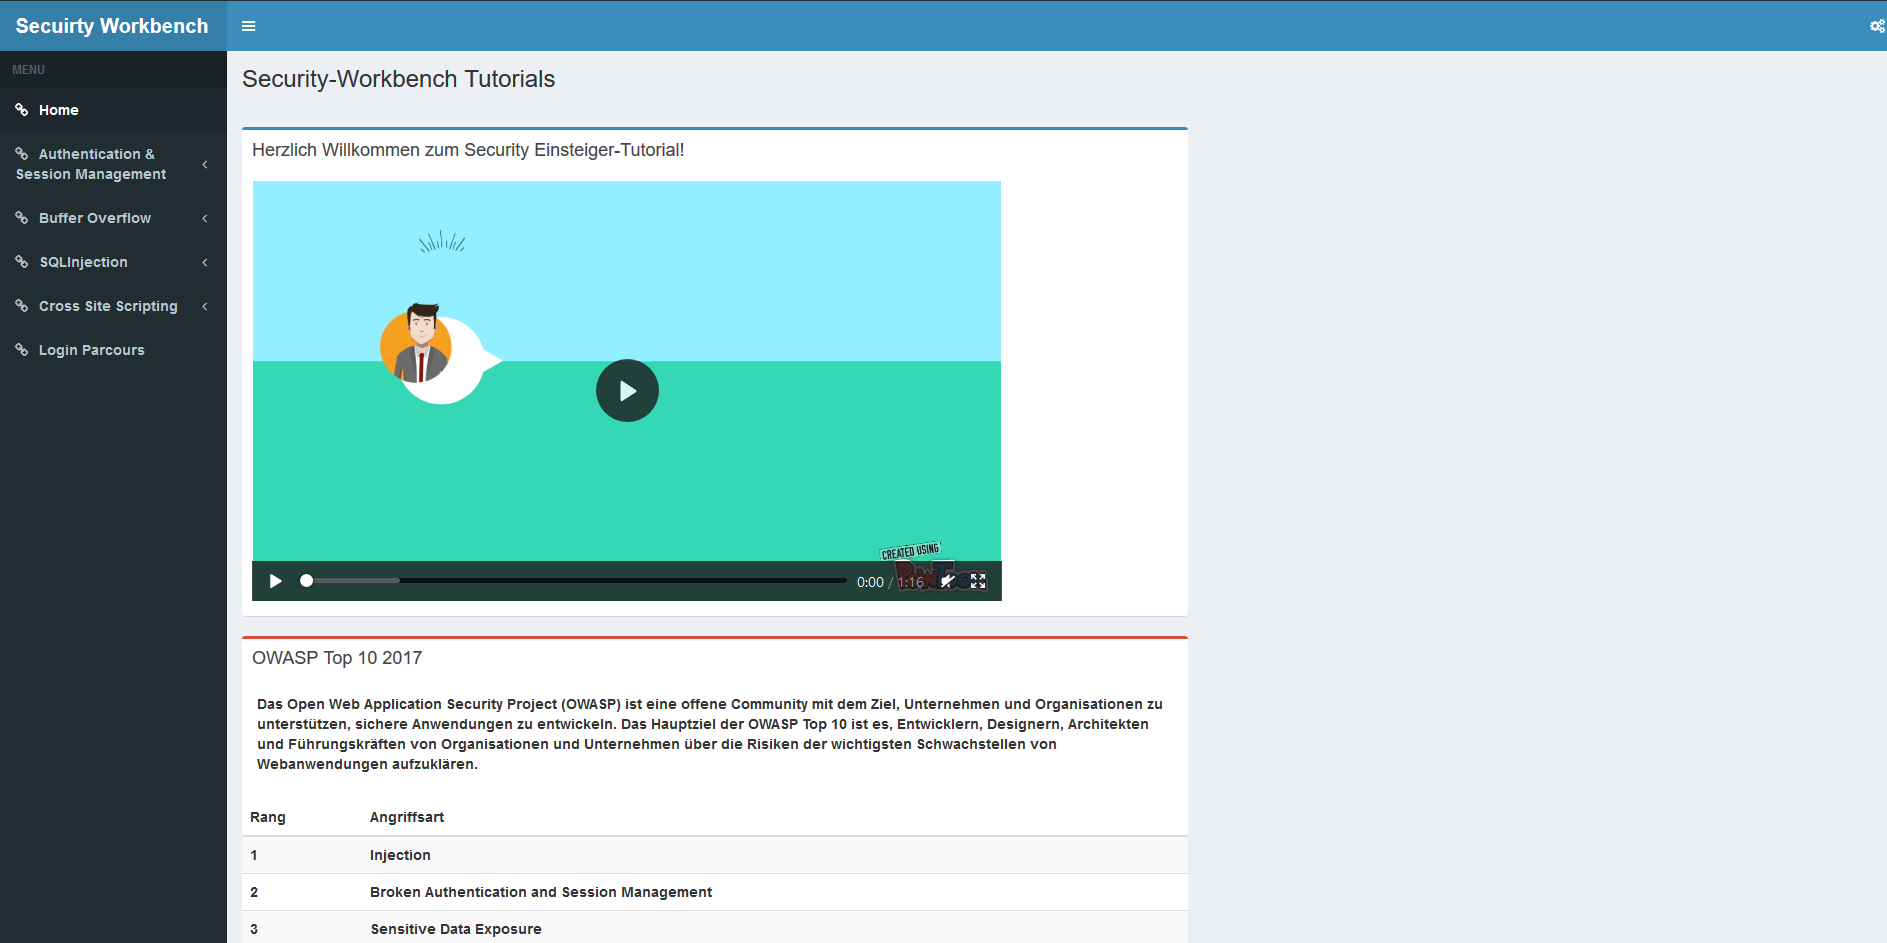
\includegraphics[width=\textwidth]{images/Installation/startseite.png}
	\caption{Nach erfolgreicher Installation, wird diese Startseite angezeigt}
	\label{fig:startseite}
\end{figure}

\section{Installationsanleitung mit Docker}
\label{sec:InstallWithDocker}

Die Installation der Web-Anwendung mithilfe des bereits konfigurierten Docker-Containers benötigt zuerst die Installation von Docker. Dies kann über den Package-Manager mit \colorbox{altgray}{\lstinline|apt-get install docker|} durchgeführt werden. Danach sollte, wie in Kapitel \ref{sec:Install} beschrieben, das GitHub-Repository geklont werden. Dort befindet sich der Ordner \colorbox{altgray}{\lstinline|PROJEKTROOT/Projekte/Docker/server |} der den Container mit allen benötigten Dienste bereitstellt. Dieses Verzeichnis muss nun auf den Desktop des Root-Users kopiert werden. Aus dem eben kopierten Ordner muss das StartUp.sh ebenfalls in das Desktop Verzeichnis verschoben werden. Dieses Skript wird dazu verwendet, den Docker-Container für die Web-Anwendung zu starten, bzw. wenn der Container noch nie gestartet wurde wird das Image des Containers erstellt. Zudem startet es alle benötigten Dienste. Es wird hier auch ein VSFTPD-Dienst gestartet. Dies ist ein FTP-Server, der nicht zwingend installiert werden muss, daher kann diese Zeile auskommentiert werden.\medskip

Nun müssen auch hier die Daten der Web-Applikation aus dem Verzeichnis \colorbox{altgray}{\lstinline|PROJEKTROOT/Projekte/SecWorkbench/html|} in den Ordner \colorbox{altgray}{\lstinline|/var/www/html|} kopiert werden. An dieser Stelle sollten die Berechtigungen mit dem Befehl \colorbox{altgray}{\lstinline|sudo chown -R www-data:www-data /var/www/html/|} aktualisiert werden. Danach kann man den Container starten, indem man das Skript StartUp.sh in der Kommandozeile aufruft. Hier sollte eine Ausgabe wie in Abbildung \ref{fig:startUp} angezeigt werden.

\begin{figure}[H]
	\centering
	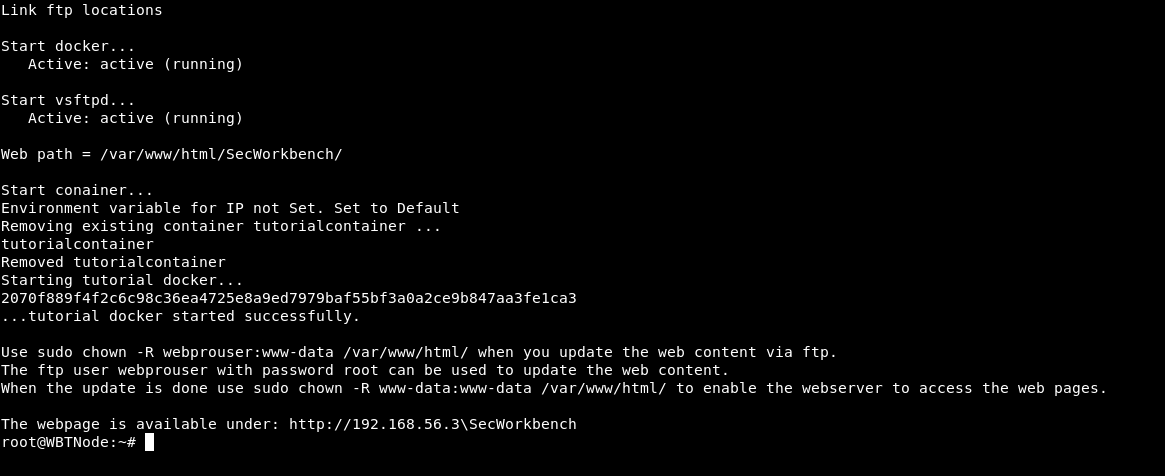
\includegraphics[width=\textwidth]{images/Installation/startUp.png}
	\caption{Die Ausgabe des Start-Skriptes nach erfolgreichem Start des Docker Containers}
	\label{fig:startUp}
\end{figure}

\section{Nutzung der virtuellen Maschine}

Die bereitgestellte virtuelle Maschine ist ein x64 Kali-Linux. Hier sind bereits alle Dienste vorinstalliert und konfiguriert. Des Weiteren wird der Root-User (ohne Passwort) automatisch beim Start der VM eingeloggt. Das Skript StartUp.sh wird beim Login des Root-Users aufgerufen, sodass die Website kurz nach dem Login erreichbar ist. Für die automatische Ausführung des Docker-Skripts dient die Konfigurationsdatei  \colorbox{altgray}{\lstinline|/root/Desktop/.config/autostart/SecWorkbench.desktop|}. Die Ausgabe des Skriptes ist in einer maximierten Shell zu sehen, dabei wird auch die URL der Web-Applikation angezeigt. Dies ist in Abbildung \ref{fig:startUp} zu sehen.\medskip

In der VM wird die Web-Anwendung in einem Docker-Container betrieben. Dieser stellt den Apache-Webserver und die MySQL-Datenbank bereit. Dadurch wird beim Starten der virtuellen Maschine immer eine initiale Datenbasis für die Tutorials bereitgestellt. Um nachsehen zu können, ob der Container richtig gestartet wurde, ist es möglich alle gestarteten Container durch das Kommando \colorbox{altgray}{\lstinline|docker ps|} anzeigen zu lassen. Hier sollte ein Container mit dem Namen tutorialcontainer mit dem Status Up zu sehen sein.\newpage

Sollte es zu einem Fehler kommen bei dem der Container abstürzt, kann dieser mit den folgenden Befehlen wieder neu gestartet werden:

\begin{enumerate}
	\item \bashCommand{docker stop tutorialcontainer}
	\item \bashCommand{docker rm tutorialcontainer}
	\item \bashCommand{'/root/Desktop/server/tutorialDockerControl.sh' start}
\end{enumerate}

Der erste Befehl stellt sicher, dass der Container gestoppt wird. Danach soll der Container gelöscht und mit dem Start-Skript neu erstellt und gestartet werden. Sollten Modifikationen am Container nötig sein, muss vor dem Neustart noch der Befehl \bashCommand{docker rmi tutorialimage} durchgeführt werden. Dieser löscht das Image, sodass aufbauend auf dem grundlegenden Debian-Images die Änderungen mit übernommen werden.\medskip

Sollten sich die Quell-Dateien ändern, so können diese über das Git-Repository aktualisiert werden. Dazu wechselt man in das Verzeichnis\\ \bashCommand{/root/INF-M-Projekt-Security-Workbench/} und führt zunächst den Befehl \bashCommand{git pull} aus. Dadurch wird das lokale Repository auf den aktuellen Stand des GitHub-Repositorys gebracht. Als nächstes kopiert man den Inhalt des Pfads \\ \bashCommand{PROJEKTROOT/Projekte/SecWorkbench/html} nach \bashCommand{/var/www/html}. Danach muss der Container gestoppt und neu gestartet werden, siehe dazu die oben stehenden Befehle 1 und 3.\medskip

In der ausgelieferten VM, kann zudem das Repository per FTP aktualisiert werden. Im startUp.sh wurden die Kommentare entfernt, die den Start des FTP-Dienstes beim Boot der VM automatisch ausführen. Dabei wird in der startUp.sh der vsftpd Dienst gestartet, indem das Kommando \bashCommand{sudo service vsftpd start} ausführt wird. Für diesen Dienst ist der User webprouser bereits eingerichtet und besitzt das Passwort root. Um Schreibrechte außerhalb des Home-Verzeichnisses des Users zu bekommen muss hier der Unterordner \bashCommand{/home/webprouser/html/SecWorkbench/} auf \bashCommand{/var/www/html/SecWorkbench/} zeigen. Dies kann mit dem Befehl\\ \bashCommand{mount --bind /home/webprouser/html/SecWorkbench/ /var/www/html/SecWorkbench/} vorgenommen werden. Um nun per FTP-Daten schreiben zu können, muss man die Berechtigungen auf dieses Verzeichnis aktualisieren. Dazu führt man das Kommando \bashCommand{sudo chown -R webprouser /home/webprouser/html/} aus. Nun können per FTP-Client Quell-Dateien direkt in das Verzeichnis, dass die HTML-Ressourcen bereitstellt eingefügt werden. Ist der Upload fertig, muss man die Rechte des html-Verzeichnisses wieder an den Apache-User geben. Dies erreicht man mit dem Befehl \bashCommand{sudo chown -R www-data:www-data /var/www/html/}.